\documentclass[11pt,letterpaper]{article}

\usepackage[utf8]{inputenc}
\usepackage[T1]{fontenc}
\usepackage[spanish,es-tabla,es-nodecimaldot,es-noquoting]{babel}
\usepackage{lmodern}
\usepackage[margin=2.5cm]{geometry}
\usepackage{amsmath,amssymb}
\usepackage{graphicx}
\usepackage{booktabs}
\usepackage{float}
\usepackage{caption}
\usepackage{subcaption}
\usepackage{algorithm}
\usepackage{algpseudocode}
\usepackage{enumitem}
\usepackage[hidelinks]{hyperref}

\graphicspath{{../figuras/}}
\captionsetup{font=small,labelfont=bf}
\floatname{algorithm}{Algoritmo}
\renewcommand{\algorithmicrequire}{\textbf{Entrada:}}
\renewcommand{\algorithmicensure}{\textbf{Salida:}}
\renewcommand{\algorithmicfor}{\textbf{para}}
\renewcommand{\algorithmicdo}{\textbf{hacer}}
\renewcommand{\algorithmicend}{\textbf{fin}}
\renewcommand{\algorithmicif}{\textbf{si}}
\renewcommand{\algorithmicthen}{\textbf{entonces}}
\renewcommand{\algorithmicelse}{\textbf{si no}}
\renewcommand{\algorithmicwhile}{\textbf{mientras}}
\renewcommand{\algorithmicreturn}{\textbf{devolver}}

\begin{document}

% ------------------------------------------------------------------
% Portada
% ------------------------------------------------------------------
\begin{titlepage}
\centering
{\large Universidad del Valle de Guatemala\par}
{\large Facultad de Ingeniería\par}
{\large Modelación y Simulación\par}
\vspace{4cm}
{\LARGE\bfseries Simulación de un sistema de atención:\\[0.3cm]
teoría de colas M/M/c y optimización\\[0.3cm] del número de cajeros\par}
\vspace{1cm}
{\large Proyecto final -- Opción 2, tema 17\par}
\vspace{4cm}
{\large
\begin{tabular}{ll}
Olivier Viau & 23544 \\
Milton Polanco & 23471 \\
\end{tabular}\par}
\vfill
{\large Guatemala, noviembre de 2026\par}
\end{titlepage}
\pagenumbering{roman}

% ------------------------------------------------------------------
\section*{Resumen}
% ------------------------------------------------------------------
En este proyecto construimos un simulador de colas por eventos discretos en Python y lo
usamos para estudiar la atención en una agencia bancaria. Primero validamos el simulador
contra las fórmulas teóricas de los modelos M/M/1, M/M/c y M/G/1; en todos los casos los
valores teóricos quedaron dentro de los intervalos de confianza del 95\,\% y los errores
relativos fueron de 4\,\% o menos. Después simulamos un día completo con llegadas que
cambian según la hora (proceso de Poisson no homogéneo generado por \emph{thinning}),
un caso en el que ya no hay fórmula exacta. Encontramos que dimensionar con la tasa
promedio subestima la espera real y que, en los días más cargados, la fila de la hora de
almuerzo pasa de 15 personas. Por último planteamos un problema de costo total (costo de cajeros más costo
de espera de los clientes). En el caso estacionario el número óptimo es $c^*=6$ cajeros, y
para el día con horas pico el mejor plan fue 4 cajeros fijos más 2 de refuerzo en los
picos, con un costo de Q2,566 por día, frente a Q3,054 de tener 5 cajeros fijos.

\newpage
\tableofcontents
\newpage
\pagenumbering{arabic}

% ------------------------------------------------------------------
\section{Introducción}
% ------------------------------------------------------------------
Las filas son parte de casi cualquier servicio: bancos, supermercados, ventanillas del
gobierno, call centers o estaciones de transporte. En todos estos casos aparece el mismo
problema: si hay pocos servidores los clientes esperan mucho, y si hay demasiados el
servicio sale caro y los empleados pasan buena parte del tiempo sin hacer nada. Decidir
cuántos servidores poner, y en qué horario, es un problema de modelación.

La teoría de colas da fórmulas cerradas para algunos modelos sencillos, pero esas fórmulas
suponen que el sistema está en estado estable y que las llegadas tienen una tasa constante.
En la práctica la demanda cambia durante el día, y ahí la simulación es la herramienta
natural. Por eso el proyecto tiene dos partes. En la primera usamos los modelos con
solución conocida para comprobar que el simulador funciona. En la segunda lo aplicamos a
un caso más realista, con horas pico, y buscamos el plan de personal de menor costo.

Los objetivos del proyecto fueron:
\begin{enumerate}[noitemsep]
  \item Implementar un simulador de colas con uno o varios servidores, con tiempos de
        llegada y de servicio generados a partir de números pseudoaleatorios.
  \item Validar el simulador contra los resultados teóricos de M/M/1, M/M/c y M/G/1.
  \item Simular un día de atención con llegadas no homogéneas y comparar distintos planes
        de personal.
  \item Encontrar el número de cajeros que minimiza el costo total, tanto en el caso
        estacionario como en el día con horas pico.
\end{enumerate}

% ------------------------------------------------------------------
\section{Descripción del fenómeno}
% ------------------------------------------------------------------
Consideramos una agencia bancaria que abre de 8:00 a 17:00. Los clientes llegan de forma
aleatoria, toman su lugar en una sola fila y pasan con el primer cajero que se desocupe
(disciplina FIFO, \emph{first in, first out}). Cada atención dura un tiempo aleatorio. Si
al llegar hay un cajero libre, el cliente pasa de inmediato; si no, espera en la fila.

El sistema es dinámico porque su estado (cuántas personas hay en la fila y qué cajeros
están ocupados) cambia con el tiempo cada vez que ocurre un evento: una llegada o el fin
de una atención. También es estocástico, porque tanto los momentos de llegada como las
duraciones de los servicios son variables aleatorias. Las preguntas que nos interesan son:
\begin{itemize}[noitemsep]
  \item ¿Cuánto espera en promedio un cliente y cuántas personas hay en la fila?
  \item ¿Qué proporción del tiempo están ocupados los cajeros?
  \item ¿Cómo cambia la espera durante el día cuando hay horas pico?
  \item ¿Cuántos cajeros conviene tener, y en qué horario, para que el costo total sea mínimo?
\end{itemize}

% ------------------------------------------------------------------
\section{Marco teórico}
% ------------------------------------------------------------------

\subsection{Proceso de Poisson y distribución exponencial}
Se dice que las llegadas forman un proceso de Poisson con tasa $\lambda$ si el número de
llegadas $N(t)$ en un intervalo de longitud $t$ cumple
\begin{equation}
  P\{N(t)=n\} = \frac{e^{-\lambda t}(\lambda t)^n}{n!}, \qquad n = 0,1,2,\dots
\end{equation}
y los conteos en intervalos disjuntos son independientes. Una consecuencia importante es
que los tiempos entre llegadas consecutivas son independientes y tienen distribución
exponencial:
\begin{equation}
  f(x) = \lambda e^{-\lambda x}, \qquad F(x) = 1 - e^{-\lambda x}, \qquad x \ge 0,
\end{equation}
con media $1/\lambda$. La exponencial es la única distribución continua sin memoria, es
decir, $P\{X > s+t \mid X > s\} = P\{X > t\}$. Esta propiedad es la que hace que los
modelos con llegadas de Poisson y servicio exponencial sean cadenas de Markov en tiempo
continuo y se puedan resolver de forma exacta.

\subsection{Notación de Kendall}
Un sistema de colas se describe con la notación $A/S/c$, donde $A$ es la distribución de
los tiempos entre llegadas, $S$ la distribución de los tiempos de servicio y $c$ el número
de servidores en paralelo. La letra M (de Markov) indica distribución exponencial y la letra
G indica una distribución general. Así, M/M/c es un sistema con llegadas de Poisson,
servicio exponencial y $c$ servidores, y M/G/1 es un sistema con llegadas de Poisson,
servicio con cualquier distribución y un solo servidor. En todos los casos supondremos
fila única, capacidad infinita y disciplina FIFO.

\subsection{Medidas de desempeño y ley de Little}
Sea $\lambda$ la tasa de llegadas, $\mu$ la tasa de servicio de cada servidor (la duración
promedio de una atención es $1/\mu$) y
\begin{equation}
  a = \frac{\lambda}{\mu}, \qquad \rho = \frac{\lambda}{c\mu},
\end{equation}
la carga ofrecida y la intensidad de tráfico (o utilización). El sistema solo es estable si
$\rho < 1$; de lo contrario la fila crece sin límite. Las medidas que usaremos son:
\begin{itemize}[noitemsep]
  \item $W_q$: tiempo promedio que un cliente espera en la fila.
  \item $W$: tiempo promedio en el sistema ($W = W_q + 1/\mu$).
  \item $L_q$: número promedio de clientes en la fila.
  \item $L$: número promedio de clientes en el sistema.
  \item $P_{\text{espera}}$: probabilidad de que un cliente tenga que esperar.
\end{itemize}
Estas medidas se relacionan por la ley de Little \cite{little}, que se cumple para
cualquier sistema estable sin importar las distribuciones:
\begin{equation}
  L = \lambda W, \qquad L_q = \lambda W_q.
\end{equation}

\subsection{Modelo M/M/1}
Con un solo servidor, el número de clientes en el sistema es un proceso de nacimiento y
muerte con probabilidades estacionarias $p_n = (1-\rho)\rho^n$. De ahí se obtiene
\cite{gross,taha}:
\begin{equation}
  L = \frac{\rho}{1-\rho}, \quad
  L_q = \frac{\rho^2}{1-\rho}, \quad
  W = \frac{1}{\mu - \lambda}, \quad
  W_q = \frac{\rho}{\mu - \lambda}, \quad
  P_{\text{espera}} = \rho.
  \label{eq:mm1}
\end{equation}

\subsection{Modelo M/M/c y fórmula de Erlang C}
Con $c$ servidores, la probabilidad de que el sistema esté vacío es
\begin{equation}
  p_0 = \left[\sum_{n=0}^{c-1} \frac{a^n}{n!} + \frac{a^c}{c!\,(1-\rho)}\right]^{-1},
\end{equation}
y la probabilidad de que un cliente que llega tenga que esperar (fórmula de Erlang C) es
\begin{equation}
  C(c,a) = P_{\text{espera}} = \frac{a^c}{c!\,(1-\rho)}\, p_0 .
\end{equation}
Con esto,
\begin{equation}
  L_q = C(c,a)\,\frac{\rho}{1-\rho}, \qquad
  W_q = \frac{L_q}{\lambda} = \frac{C(c,a)}{c\mu - \lambda}, \qquad
  W = W_q + \frac{1}{\mu}, \qquad L = \lambda W .
  \label{eq:mmc}
\end{equation}
Para $c=1$ estas expresiones se reducen a las de M/M/1. Además, en M/M/c el tiempo de
espera de quienes esperan es exponencial con tasa $c\mu-\lambda$, por lo que
\begin{equation}
  P\{W_q > t\} = C(c,a)\, e^{-(c\mu - \lambda)t}, \qquad t \ge 0.
  \label{eq:colawq}
\end{equation}

\subsection{Modelo M/G/1 y aproximación para M/G/c}
Si el servicio tiene una distribución cualquiera con media $E[S]$ y varianza
$\operatorname{Var}(S)$, el tiempo de espera en M/G/1 está dado por la fórmula de
Pollaczek-Khinchine \cite{gross}:
\begin{equation}
  W_q = \frac{\lambda\, E[S^2]}{2(1-\rho)}
      = \frac{\lambda\left(\operatorname{Var}(S) + E[S]^2\right)}{2(1-\rho)}
      = \frac{\rho\,E[S]}{1-\rho}\cdot\frac{1 + C_s^2}{2},
  \label{eq:pk}
\end{equation}
donde $C_s^2 = \operatorname{Var}(S)/E[S]^2$ es el coeficiente de variación al cuadrado del
servicio. Para la exponencial $C_s^2=1$ y se recupera $W_q$ de M/M/1; para un servicio
determinista $C_s^2 = 0$ y la espera se reduce a la mitad.

Para M/G/c no existe una fórmula exacta. Una aproximación muy usada es la de
Allen-Cunneen \cite{allen}:
\begin{equation}
  W_q(\text{M/G/}c) \approx W_q(\text{M/M/}c)\cdot\frac{1 + C_s^2}{2}.
  \label{eq:ac}
\end{equation}

\subsection{Proceso de Poisson no homogéneo}
Cuando la tasa de llegadas depende del tiempo, $\lambda = \lambda(t)$, el número de
llegadas en $[s,t]$ es Poisson con media $\Lambda(s,t) = \int_s^t \lambda(u)\,du$. En este
caso las fórmulas anteriores ya no aplican, porque el sistema no llega a un estado
estable: la fila responde con retraso a los cambios en la demanda. Una práctica común es
evaluar las fórmulas estacionarias con la tasa promedio o con la tasa de cada hora, pero
se sabe que esto puede dar resultados engañosos cuando la demanda es cíclica
\cite{green}. Esto es justo lo que estudiamos en el escenario 3.

% ------------------------------------------------------------------
\section{Métodos de simulación}
% ------------------------------------------------------------------
Todo el código está escrito en Python, con \texttt{numpy} para la generación de números
aleatorios y el manejo de arreglos, \texttt{scipy} para las pruebas estadísticas y
\texttt{matplotlib} para las gráficas. Todas las tasas se trabajan en clientes por minuto
y todos los tiempos en minutos.

\subsection{Generación de números aleatorios}
Como generador base usamos el Mersenne Twister (MT19937) \cite{mt}, el mismo que
estudiamos en el laboratorio 2, a través de \texttt{np.random.MT19937}. Cada réplica
usa una semilla distinta para que las réplicas sean independientes y los resultados se
puedan reproducir.

Los tiempos exponenciales se generan con el método de la transformada inversa
\cite{ross}. Si $U \sim \text{Unif}(0,1)$, entonces despejando $u = F(x) = 1-e^{-\lambda x}$
se obtiene
\begin{equation}
  X = F^{-1}(U) = -\frac{\ln(1-U)}{\lambda} \sim \text{Exp}(\lambda).
\end{equation}
Las llegadas de un proceso de Poisson homogéneo en $[0,T]$ se obtienen como sumas
acumuladas de tiempos entre llegadas exponenciales hasta pasar $T$. Para los escenarios
con servicio no exponencial se usaron la distribución uniforme, la gamma y un servicio
determinista, todas con la misma media.

\subsection{Simulación de la cola por eventos discretos}
Con disciplina FIFO y servidores idénticos, no hace falta una lista general de eventos.
Basta con guardar, para cada servidor, el instante en que se desocupa. Cada cliente, en
orden de llegada, pasa con el servidor que se libere primero; si llega antes de ese
momento espera, y si llega después lo atienden de inmediato. Guardamos los instantes de
desocupación en un \emph{heap} (montículo), de modo que obtener el servidor que se libera
primero cuesta $O(\log c)$.

\begin{algorithm}[H]
\caption{Simulación de una cola FIFO con $c$ servidores}
\label{alg:cola}
\begin{algorithmic}[1]
\Require llegadas $a_1 \le a_2 \le \dots \le a_n$, servicios $s_1,\dots,s_n$, número de servidores $c$
\Ensure inicio de servicio $b_i$ y salida $d_i$ de cada cliente
\State $H \gets$ heap con $c$ ceros \Comment{momento en que se libera cada servidor}
\For{$i = 1, \dots, n$}
  \State $t \gets$ extraer el mínimo de $H$
  \State $b_i \gets \max(a_i, t)$ \Comment{espera si el servidor sigue ocupado}
  \State $d_i \gets b_i + s_i$
  \State insertar $d_i$ en $H$
\EndFor
\State \Return $b, d$
\end{algorithmic}
\end{algorithm}

Para el día con horas pico se necesitan cajeros que solo trabajan en ciertos horarios.
En ese caso cada servidor $k$ tiene una lista de turnos $[(e_1,f_1),(e_2,f_2),\dots]$ y,
para cada cliente, calculamos el primer instante en que cada servidor está libre
\emph{y} dentro de un turno; el cliente pasa con el que dé el menor instante. Un cajero no
empieza a atender después del fin de su turno, pero sí termina al cliente que ya tenía.
Como los clientes se procesan en orden de llegada y cada uno toma el mínimo, se conserva
la disciplina FIFO.

\subsection{Llegadas no homogéneas: método de \emph{thinning}}
Para generar un proceso de Poisson con tasa $\lambda(t)$ usamos el método de
\emph{thinning} de Lewis y Shedler \cite{lewis}. Es una forma de aceptación y rechazo,
como la que usamos en el laboratorio 3: se generan llegadas candidatas con una tasa
constante $\lambda_{\max} \ge \lambda(t)$ y cada una se acepta con probabilidad
$\lambda(t)/\lambda_{\max}$.

\begin{algorithm}[H]
\caption{\emph{Thinning} para un proceso de Poisson no homogéneo}
\label{alg:thinning}
\begin{algorithmic}[1]
\Require función $\lambda(t)$, cota $\lambda_{\max}$, horizonte $T$
\State generar un proceso de Poisson homogéneo $t_1 < t_2 < \dots < t_m$ en $[0,T]$ con tasa $\lambda_{\max}$
\For{$j = 1, \dots, m$}
  \State generar $U_j \sim \text{Unif}(0,1)$
  \If{$U_j \le \lambda(t_j)/\lambda_{\max}$}
    \State aceptar $t_j$ como llegada
  \EndIf
\EndFor
\State \Return las llegadas aceptadas
\end{algorithmic}
\end{algorithm}

La proporción esperada de candidatas aceptadas es
$\bar{\lambda}/\lambda_{\max}$, donde $\bar\lambda$ es la tasa promedio en $[0,T]$. Esto
nos sirve para revisar que el método está bien implementado.

\subsection{Cálculo de las medidas de desempeño}
Una vez simulada una corrida, $W_q$ y $W$ se calculan como el promedio de
$b_i - a_i$ y $d_i - a_i$ de los clientes que llegaron dentro de la ventana de
observación $[t_0, t_1]$. Las medidas $L_q$, $L$ y la utilización son promedios en el
tiempo; por ejemplo,
\begin{equation}
  L_q = \frac{1}{t_1 - t_0}\int_{t_0}^{t_1} N_q(t)\,dt
      = \frac{1}{t_1 - t_0}\sum_i \bigl|[a_i, b_i] \cap [t_0, t_1]\bigr| ,
\end{equation}
ya que cada cliente aporta a la integral exactamente el tiempo que pasa en la fila dentro
de la ventana. De la misma forma se obtienen $L$ (con $[a_i,d_i]$) y la utilización (con
$[b_i,d_i]$, dividiendo además entre $c$). Calcular $L_q$ de esta forma y no con la ley de
Little nos permite usar la ley como una prueba independiente del simulador.

\subsection{Diseño estadístico}
Para cada configuración corremos $R$ réplicas independientes y reportamos la media
$\bar{X}$ con su intervalo de confianza del 95\,\%:
\begin{equation}
  \bar{X} \pm t_{0.975,\,R-1}\,\frac{S}{\sqrt{R}},
\end{equation}
donde $S$ es la desviación estándar entre réplicas. En los escenarios estacionarios el
sistema arranca vacío, lo cual introduce un sesgo al inicio. Para eliminarlo descartamos
un periodo de calentamiento (alrededor del 10\,\% del horizonte) antes de medir. En la
comparación de planes de personal usamos números aleatorios comunes: todos los planes se
evalúan con los mismos días simulados (mismas llegadas y mismos servicios), así las
diferencias se deben al plan y no al azar, y se pueden comparar con una prueba pareada.

% ------------------------------------------------------------------
\section{Metodología}
% ------------------------------------------------------------------
Diseñamos cinco escenarios. Los dos primeros sirven para validar el simulador, el tercero
y el cuarto exploran casos donde las fórmulas exactas ya no aplican y el quinto resuelve
el problema de optimización. La Tabla~\ref{tab:escenarios} resume los parámetros.

\begin{table}[H]
\centering
\caption{Escenarios simulados.}
\label{tab:escenarios}
\small
\begin{tabular}{@{}clllc@{}}
\toprule
Esc. & Modelo & Llegadas & Servicio (media) & Réplicas / horizonte \\
\midrule
1 & M/M/1 & Poisson, 20 cl/h & Exp., 2.5 min & 30 $\times$ 10{,}000 min \\
  & & ($\rho$ de 0.3 a 0.95) & & 30 $\times$ 40{,}000--150{,}000 min \\
2 & M/M/$c$, $c=5,\dots,8$ & Poisson, 50 cl/h & Exp., 5 min & 30 $\times$ 20{,}000 min \\
3 & M$_t$/M/$c(t)$ & Poisson no homogéneo & Exp., 5 min & 50 días de 540 min \\
4 & M/G/1 y M/G/5 & Poisson, 20 y 50 cl/h & 6 distribuciones & 30 $\times$ 40{,}000 min \\
5 & Optimización & como esc. 2 y 3 & Exp., 5 min & 30 réplicas / 50 días \\
\bottomrule
\end{tabular}
\end{table}

\paragraph{Escenario 1 (M/M/1).} Una sola caja con 20 clientes por hora y atención promedio
de 2.5 minutos, lo que da $\rho = 0.833$. Además de comparar todas las medidas con
\eqref{eq:mm1}, aplicamos pruebas de Kolmogorov-Smirnov y $\chi^2$ a los tiempos generados
y hacemos un barrido de $\rho$ entre 0.3 y 0.95. Para $\rho \ge 0.85$ usamos corridas de
150{,}000 minutos con 15{,}000 de calentamiento, porque cerca de la saturación el sistema
tarda mucho más en llegar al estado estable.

\paragraph{Escenario 2 (M/M/$c$).} 50 clientes por hora y atención de 5 minutos, es decir,
$a = 4.17$; se necesitan al menos 5 cajas para que el sistema sea estable. Comparamos
$c = 5,6,7,8$ con \eqref{eq:mmc} y \eqref{eq:colawq}. También comparamos, con 6 cajas, una
fila única contra una fila por caja donde cada cliente escoge una caja al azar.

\paragraph{Escenario 3 (horas pico).} La agencia abre 540 minutos (8:00 a 17:00) y la tasa
de llegadas es una base de 27 clientes por hora más tres picos gaussianos:
\begin{equation}
  \lambda(t) = 0.45 + 0.45\,e^{-\frac{(t-90)^2}{2\cdot 35^2}}
                    + 0.65\,e^{-\frac{(t-285)^2}{2\cdot 40^2}}
                    + 0.45\,e^{-\frac{(t-495)^2}{2\cdot 35^2}}
  \quad \text{clientes/min},
\end{equation}
con $t$ en minutos desde la apertura. Los picos quedan a las 9:30, 12:45 y 16:15, con
54, 66 y 54 clientes por hora. La tasa promedio es 42.6 clientes por hora (unos 383
clientes al día). Usamos $\lambda_{\max} = 1.2$ clientes/min para el \emph{thinning}.
Comparamos cuatro planes de personal; los cajeros de refuerzo trabajan solo en las
ventanas 8:45--10:30, 11:45--13:45 y 15:15--17:00 (5.5 horas al día cada uno). Las
puertas cierran a las 17:00, pero quienes ya están en la fila sí son atendidos.

\paragraph{Escenario 4 (servicio no exponencial).} Mantenemos la media del servicio y
cambiamos su variabilidad: determinista ($C_s^2=0$), uniforme en $[0.2m, 1.8m]$
($C_s^2=0.213$), gamma con forma $k=2$ ($C_s^2=0.5$), exponencial ($C_s^2=1$) y gamma con
$k=0.5$ y $k=0.25$ ($C_s^2 = 2$ y $4$). Con un servidor comparamos con \eqref{eq:pk}, y con 5
servidores con la aproximación \eqref{eq:ac}.

\paragraph{Escenario 5 (optimización).} Planteamos el costo total como la suma del costo
de los cajeros más el costo de la espera de los clientes. Suponemos que un cajero cuesta
$C_s = \text{Q}45$ por hora (salario y prestaciones) y que cada hora que un cliente pasa en
la fila tiene un costo $C_w = \text{Q}60$, que representa el tiempo perdido del cliente y
el riesgo de que se cambie de banco. En el caso estacionario del escenario 2 el costo por
hora es
\begin{equation}
  CT(c) = C_s\, c + C_w\, L_q(c),
\end{equation}
y buscamos el $c$ que lo minimiza. Como $C_w$ es difícil de estimar, hacemos también un
análisis de sensibilidad respecto a la razón $C_w/C_s$. Para el día con horas pico el costo
diario es
\begin{equation}
  CT = C_s \cdot (\text{horas-cajero}) + C_w \cdot \sum_i W_{q,i},
\end{equation}
donde la suma es el total de horas de espera de todos los clientes del día. Evaluamos
todas las combinaciones de 3 a 6 cajeros fijos con 0 a 3 de refuerzo (16 planes).

% ------------------------------------------------------------------
\section{Resultados}
% ------------------------------------------------------------------

\subsection{Escenario 1: validación con M/M/1}

\paragraph{Números aleatorios.} Antes de simular la cola revisamos que los tiempos
generados realmente fueran exponenciales. La Tabla~\ref{tab:ajuste} muestra que ninguna de
las pruebas rechaza la hipótesis nula con $\alpha = 0.05$, y la Figura~\ref{fig:hist}
muestra que los histogramas siguen la densidad teórica.

\begin{table}[H]
\centering
\caption{Pruebas de bondad de ajuste a la distribución exponencial ($\chi^2$ con 10 clases equiprobables).}
\label{tab:ajuste}
\small
\begin{tabular}{@{}lrrrrrrr@{}}
\toprule
Variable & $n$ & Media & Media teórica & $D$ (KS) & $p$ KS & $\chi^2$ & $p$ $\chi^2$ \\
\midrule
Entre llegadas & 20{,}073 & 2.989 & 3.000 & 0.0051 & 0.665 & 4.330 & 0.888 \\
Servicio       & 20{,}000 & 2.505 & 2.500 & 0.0052 & 0.652 & 4.691 & 0.860 \\
\bottomrule
\end{tabular}
\end{table}

\begin{figure}[H]
\centering
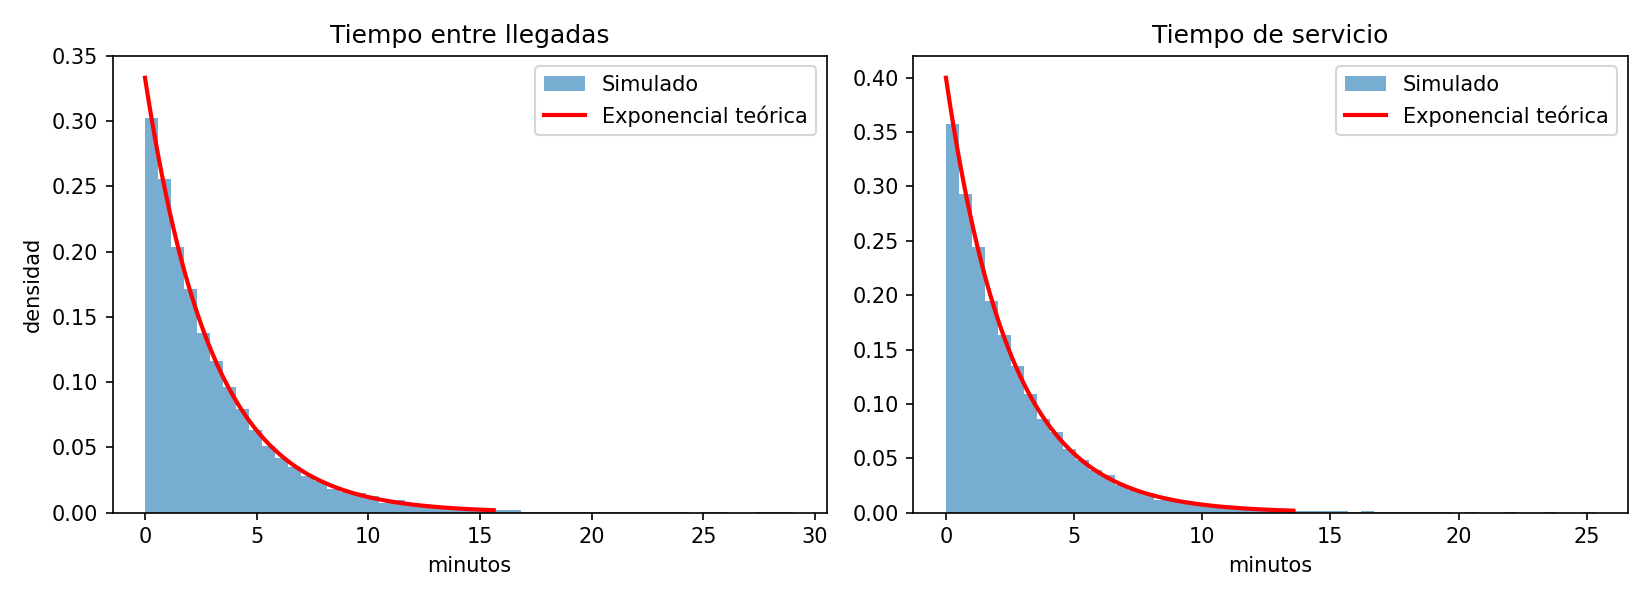
\includegraphics[width=0.95\textwidth]{esc1_histogramas.png}
\caption{Histogramas de los tiempos generados por transformada inversa y densidad exponencial teórica.}
\label{fig:hist}
\end{figure}

\paragraph{Simulación contra teoría.} La Tabla~\ref{tab:mm1} compara las medidas simuladas
con las de \eqref{eq:mm1}. Todos los valores teóricos están dentro del intervalo de
confianza y los errores relativos son menores al 4.1\,\%. La utilización y la probabilidad
de espera tienen errores menores al 1\,\%. También se cumple la ley de Little: el $L$
medido como promedio en el tiempo fue 5.1739 y $\lambda W$ dio 5.1741.

\begin{table}[H]
\centering
\caption{M/M/1 con $\lambda = 20$ cl/h y $\mu = 24$ cl/h ($\rho = 0.833$), 30 réplicas. Tiempos en minutos.}
\label{tab:mm1}
\small
\begin{tabular}{@{}lrrrr@{}}
\toprule
Medida & Teórico & Simulado & IC 95\,\% ($\pm$) & Error (\%) \\
\midrule
$W_q$ & 12.500 & 12.965 & 1.014 & 3.72 \\
$W$ & 15.000 & 15.478 & 1.025 & 3.19 \\
$L_q$ & 4.167 & 4.335 & 0.351 & 4.04 \\
$L$ & 5.000 & 5.174 & 0.358 & 3.48 \\
Utilización & 0.833 & 0.839 & 0.009 & 0.68 \\
$P_{\text{espera}}$ & 0.833 & 0.839 & 0.010 & 0.65 \\
\bottomrule
\end{tabular}
\end{table}

\paragraph{Barrido de $\rho$.} La Figura~\ref{fig:barrido} y la Tabla~\ref{tab:barrido}
muestran $W_q$ para distintas intensidades de tráfico. La simulación sigue la curva
teórica en todo el rango y el error máximo fue 3.1\,\%. Algo que observamos es que el
intervalo de confianza crece mucho cuando $\rho$ se acerca a 1: con $\rho = 0.95$ el
ancho es $\pm 3$ minutos aun con corridas de 150{,}000 minutos. En nuestras primeras
pruebas, con corridas de 40{,}000 minutos y poco calentamiento, la simulación
subestimaba $W_q$ en casi 10\,\% para $\rho = 0.95$, porque el sistema arrancaba vacío y
no alcanzaba a llegar al estado estable.

\begin{table}[H]
\centering
\caption{$W_q$ (min) en M/M/1 para distintos valores de $\rho$ (30 réplicas cada uno).}
\label{tab:barrido}
\small
\begin{tabular}{@{}rrrrrr@{}}
\toprule
$\rho$ & $\lambda$ (cl/h) & $W_q$ teórico & $W_q$ simulado & IC 95\,\% ($\pm$) & Error (\%) \\
\midrule
0.30 & 7.2 & 1.071 & 1.055 & 0.023 & 1.53 \\
0.50 & 12.0 & 2.500 & 2.494 & 0.061 & 0.24 \\
0.60 & 14.4 & 3.750 & 3.729 & 0.111 & 0.55 \\
0.70 & 16.8 & 5.833 & 5.911 & 0.208 & 1.33 \\
0.80 & 19.2 & 10.000 & 9.686 & 0.367 & 3.14 \\
0.85 & 20.4 & 14.167 & 14.093 & 0.385 & 0.52 \\
0.90 & 21.6 & 22.500 & 22.876 & 0.705 & 1.67 \\
0.95 & 22.8 & 47.500 & 47.880 & 3.046 & 0.80 \\
\bottomrule
\end{tabular}
\end{table}

\begin{figure}[H]
\centering
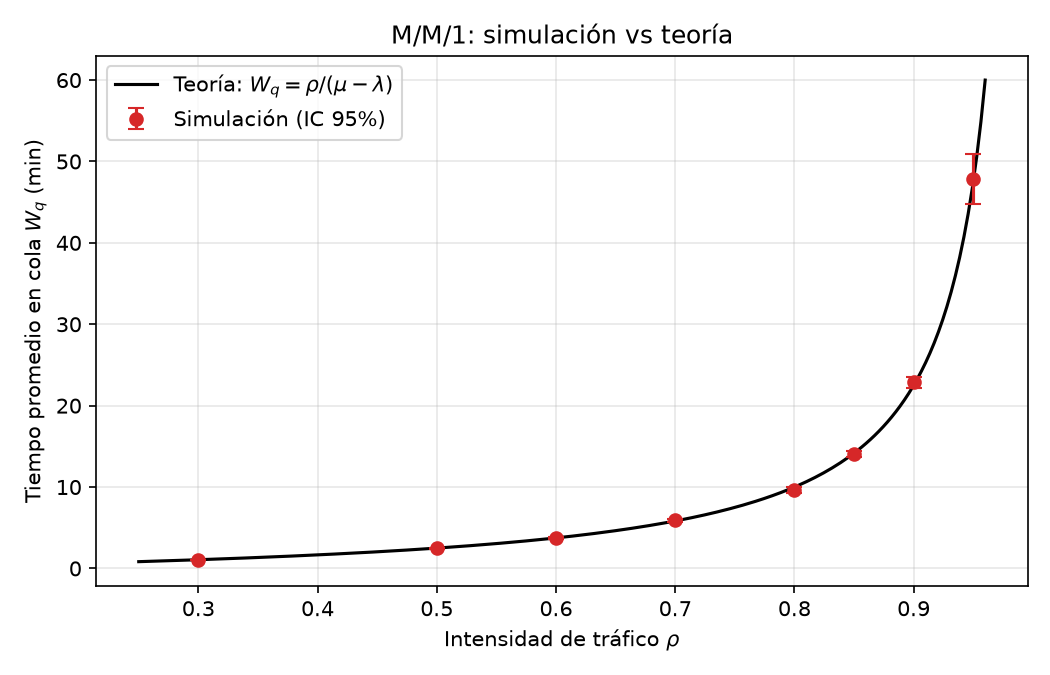
\includegraphics[width=0.7\textwidth]{esc1_barrido_rho.png}
\caption{Tiempo promedio en cola de M/M/1 en función de $\rho$: teoría y simulación.}
\label{fig:barrido}
\end{figure}

La Figura~\ref{fig:mm1tiempo} muestra una sola jornada de 8 horas. Aunque el promedio
teórico de la fila es 4.2 personas, en un día concreto la fila varía mucho: al inicio casi
no hay nadie y unas seis horas después llega a 17 personas. Esto es normal cuando $\rho$ es alto y es una de las
razones por las que hay que usar varias réplicas para estimar promedios.

\begin{figure}[H]
\centering
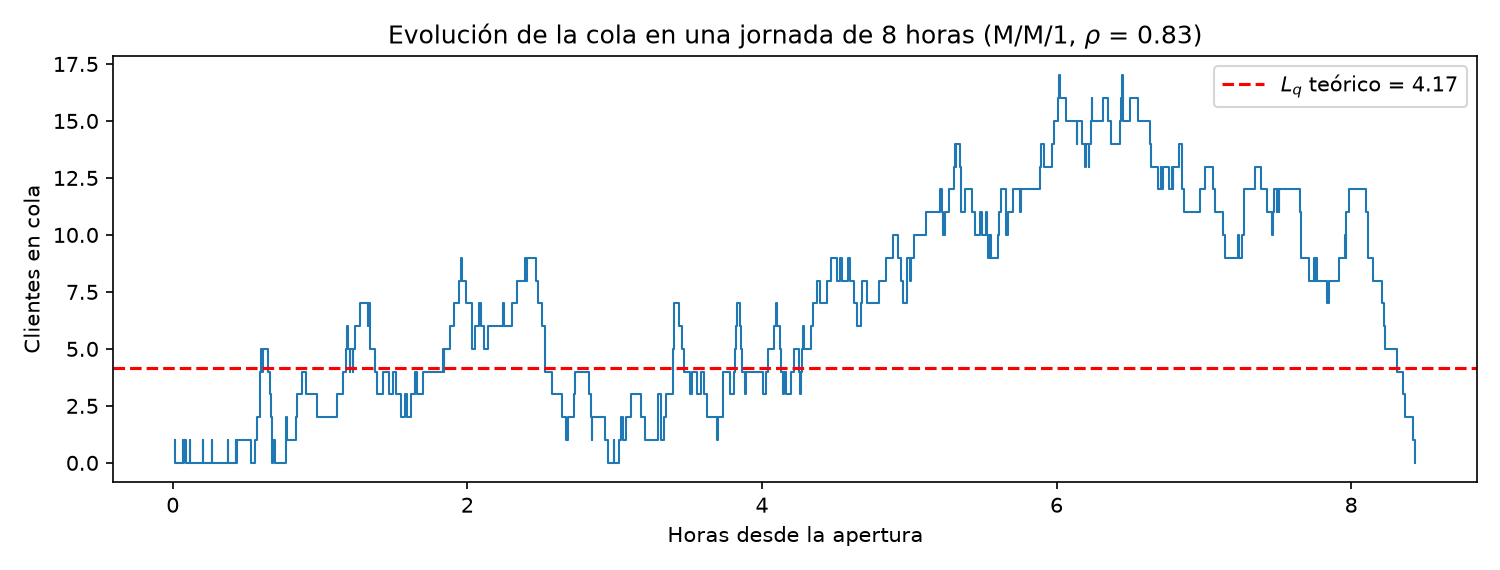
\includegraphics[width=0.95\textwidth]{esc1_cola_tiempo.png}
\caption{Número de clientes en la fila durante una jornada simulada de M/M/1.}
\label{fig:mm1tiempo}
\end{figure}

\subsection{Escenario 2: varias cajas (\texorpdfstring{M/M/$c$}{M/M/c})}
La Tabla~\ref{tab:mmc} muestra la comparación con las fórmulas de Erlang C. Para todos los
valores de $c$ los errores de $W_q$ y $L_q$ están por debajo de 2.4\,\% y los de la
utilización por debajo de 0.04\,\%. Con 5 cajas el 62\,\% de los clientes tiene que esperar;
con 6 cajas esa proporción baja a 33\,\% y $W_q$ cae de 3.8 a 0.9 minutos. Es decir, la
sexta caja es la que tiene más impacto; a partir de ahí cada caja adicional mejora cada vez
menos.

\begin{table}[H]
\centering
\caption{M/M/$c$ con $\lambda = 50$ cl/h y servicio de 5 min, 30 réplicas.}
\label{tab:mmc}
\small
\begin{tabular}{@{}crrrrrrr@{}}
\toprule
$c$ & $\rho$ & \multicolumn{2}{c}{$P_{\text{espera}}$} & \multicolumn{2}{c}{$W_q$ (min)} & \multicolumn{2}{c}{$L_q$} \\
\cmidrule(lr){3-4}\cmidrule(lr){5-6}\cmidrule(l){7-8}
 & & Teórico & Simulado & Teórico & Simulado & Teórico & Simulado \\
\midrule
5 & 0.833 & 0.620 & 0.622 & 3.721 & 3.807 & 3.101 & 3.173 \\
6 & 0.694 & 0.327 & 0.327 & 0.892 & 0.901 & 0.743 & 0.751 \\
7 & 0.595 & 0.160 & 0.160 & 0.282 & 0.286 & 0.235 & 0.238 \\
8 & 0.521 & 0.072 & 0.072 & 0.094 & 0.096 & 0.078 & 0.080 \\
\bottomrule
\end{tabular}
\end{table}

\begin{figure}[H]
\centering
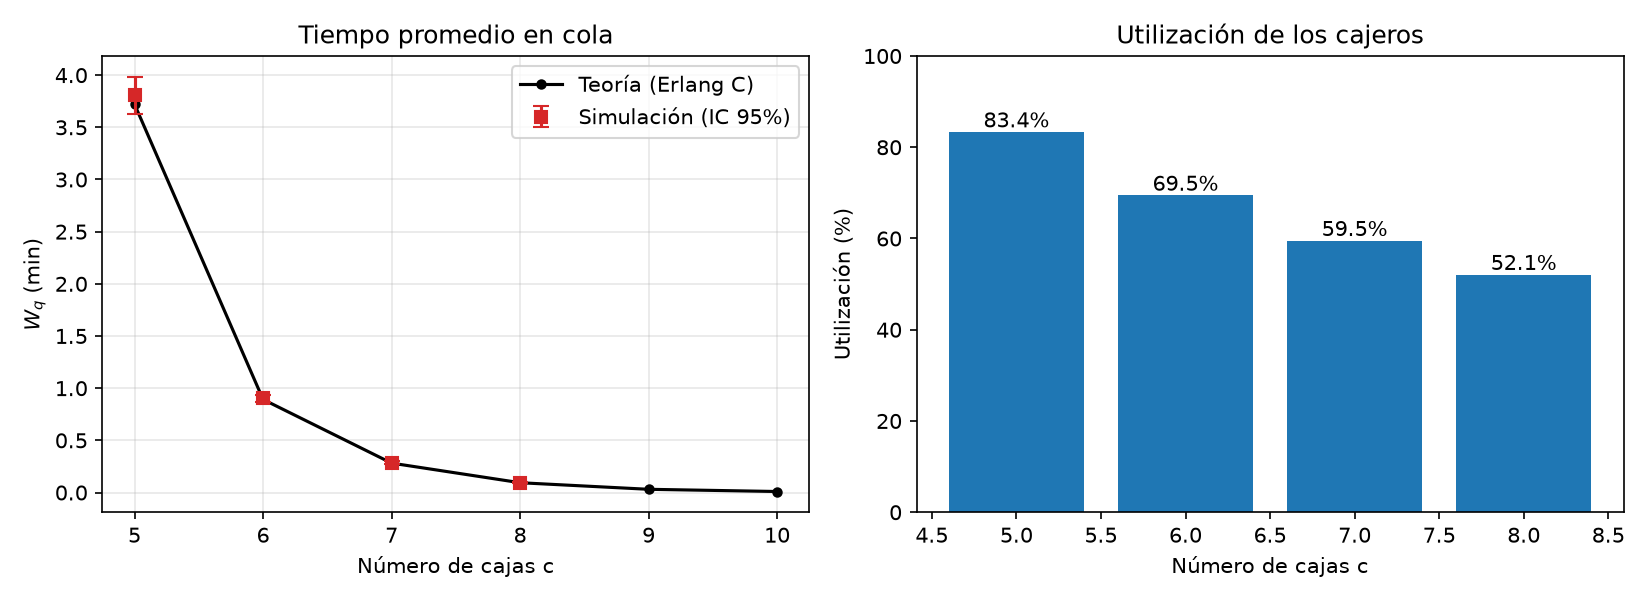
\includegraphics[width=0.95\textwidth]{esc2_wq_utilizacion.png}
\caption{Izquierda: $W_q$ según el número de cajas. Derecha: utilización de los cajeros.}
\label{fig:mmc}
\end{figure}

La Figura~\ref{fig:distesp} compara la distribución completa del tiempo de espera con
\eqref{eq:colawq}. En escala logarítmica la teoría es una recta, y la simulación la sigue
bien hasta probabilidades de alrededor de 1\,\%. Más allá, en la cola de la distribución,
la curva simulada para $c=5$ queda un poco por encima; ahí hay muy pocos datos y las
esperas largas vienen en grupos (cuando la fila crece afecta a muchos clientes seguidos),
por lo que la estimación es menos precisa.

\begin{figure}[H]
\centering
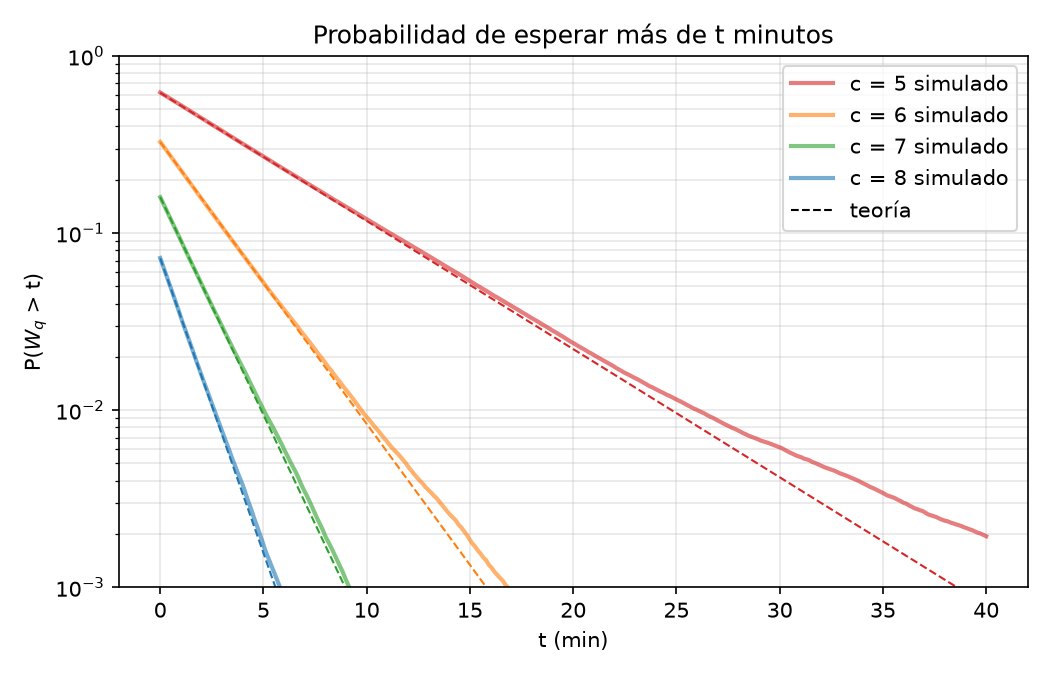
\includegraphics[width=0.7\textwidth]{esc2_distribucion_espera.png}
\caption{Probabilidad de esperar más de $t$ minutos. Línea continua: simulación; línea punteada: ecuación \eqref{eq:colawq}.}
\label{fig:distesp}
\end{figure}

\paragraph{Fila única contra una fila por caja.} Con las mismas 6 cajas, organizar a los
clientes en una sola fila en lugar de una fila por caja cambia por completo el resultado
(Tabla~\ref{tab:filas} y Figura~\ref{fig:filas}). Con filas separadas cada caja se comporta
como un M/M/1 con $\rho = 0.69$, y una caja puede quedar libre mientras en otra hay gente
esperando. Con fila única eso no pasa. La espera promedio baja de 11.5 a 0.9 minutos y el
porcentaje de clientes que espera más de 10 minutos baja de 38\,\% a menos de 1\,\%.

\begin{table}[H]
\centering
\caption{Fila única contra una fila por caja con $c = 6$.}
\label{tab:filas}
\small
\begin{tabular}{@{}lrrr@{}}
\toprule
Sistema & $W_q$ teórico (min) & $W_q$ simulado (min) & \% que espera $>10$ min \\
\midrule
Una fila por caja ($6\times$M/M/1) & 11.364 & 11.547 & 37.96 \\
Fila única (M/M/6) & 0.892 & 0.894 & 0.88 \\
\bottomrule
\end{tabular}
\end{table}

\begin{figure}[H]
\centering
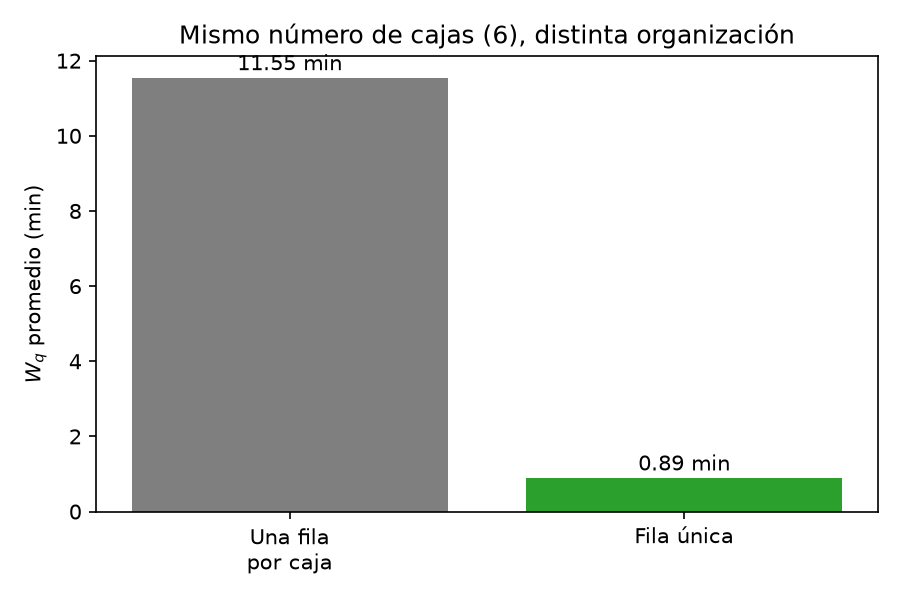
\includegraphics[width=0.5\textwidth]{esc2_fila_unica_vs_separadas.png}
\caption{Espera promedio con la misma cantidad de cajas y distinta organización de la fila.}
\label{fig:filas}
\end{figure}

\subsection{Escenario 3: un día con horas pico}
La Figura~\ref{fig:tasa} muestra la tasa de llegadas $\lambda(t)$ junto con el número
promedio de llegadas simuladas en intervalos de 15 minutos. Las barras siguen la curva,
lo que confirma que el \emph{thinning} genera el proceso correcto. La proporción de
candidatas aceptadas fue 0.5884, muy cerca del valor teórico
$\bar\lambda/\lambda_{\max} = 0.5911$.

\begin{figure}[H]
\centering
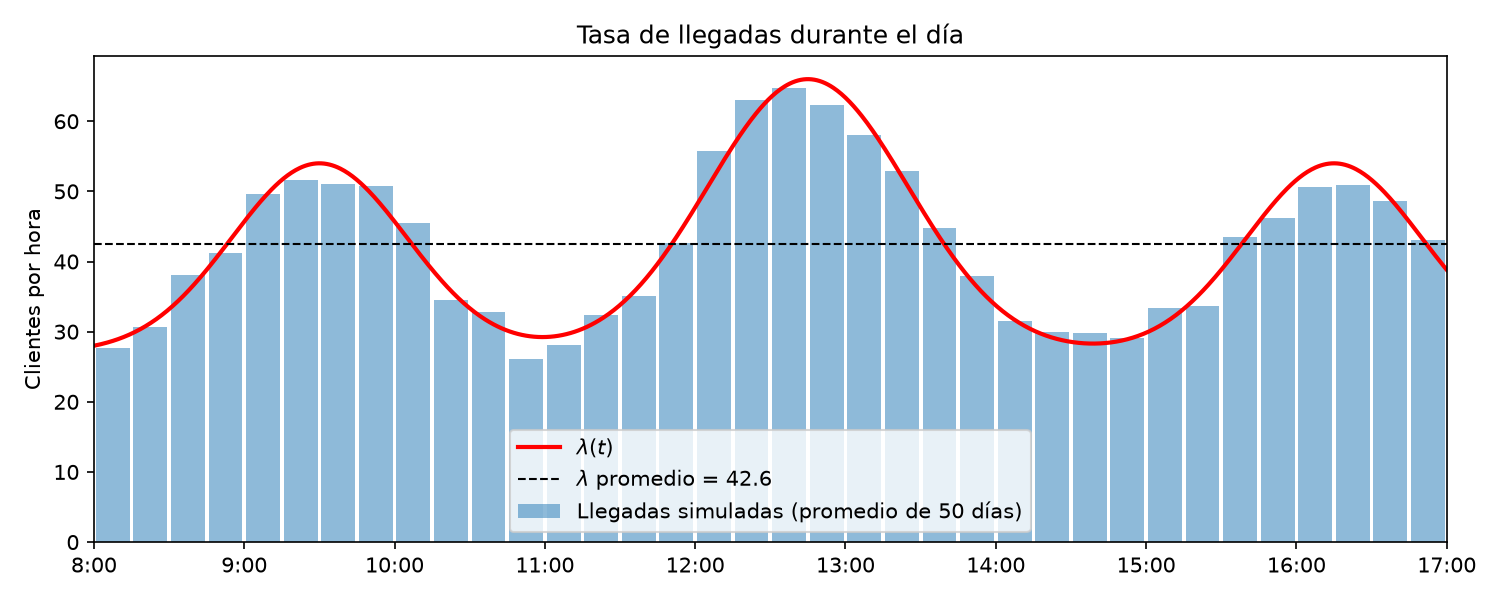
\includegraphics[width=0.95\textwidth]{esc3_tasa_llegadas.png}
\caption{Tasa de llegadas $\lambda(t)$ y llegadas simuladas por hora (promedio de 50 días).}
\label{fig:tasa}
\end{figure}

\paragraph{¿Sirve la fórmula con la tasa promedio?} Si se usa M/M/$c$ con
$\bar\lambda = 42.6$ cl/h, la fórmula dice que con 5 cajas la espera promedio sería 1.35
minutos. La simulación del día completo da $2.39 \pm 0.38$ minutos, casi el doble. El
problema es que el promedio esconde los picos: entre 12:22 y 13:08 llegan más de 60
clientes por hora y 5 cajas solo pueden atender 60, así que durante ese rato el sistema
está saturado ($\rho > 1$).

La Figura~\ref{fig:coladia} muestra otra limitación. Ahí se compara la fila simulada con
lo que daría la fórmula de M/M/5 evaluada en cada instante con $\lambda(t)$. La fórmula
se va a infinito en el pico del almuerzo y luego cae rápido, mientras que la fila real
crece más despacio, llega a su máximo después del pico de llegadas (alrededor de las
13:15) y tarda casi una hora en vaciarse. La fila tiene ``memoria'': los clientes que se
acumularon en el pico siguen ahí aunque la tasa de llegadas ya haya bajado. Ninguna
fórmula estacionaria captura ese retraso. En el 10\,\% de los días más cargados la fila
pasa de 15 personas.

\begin{figure}[H]
\centering
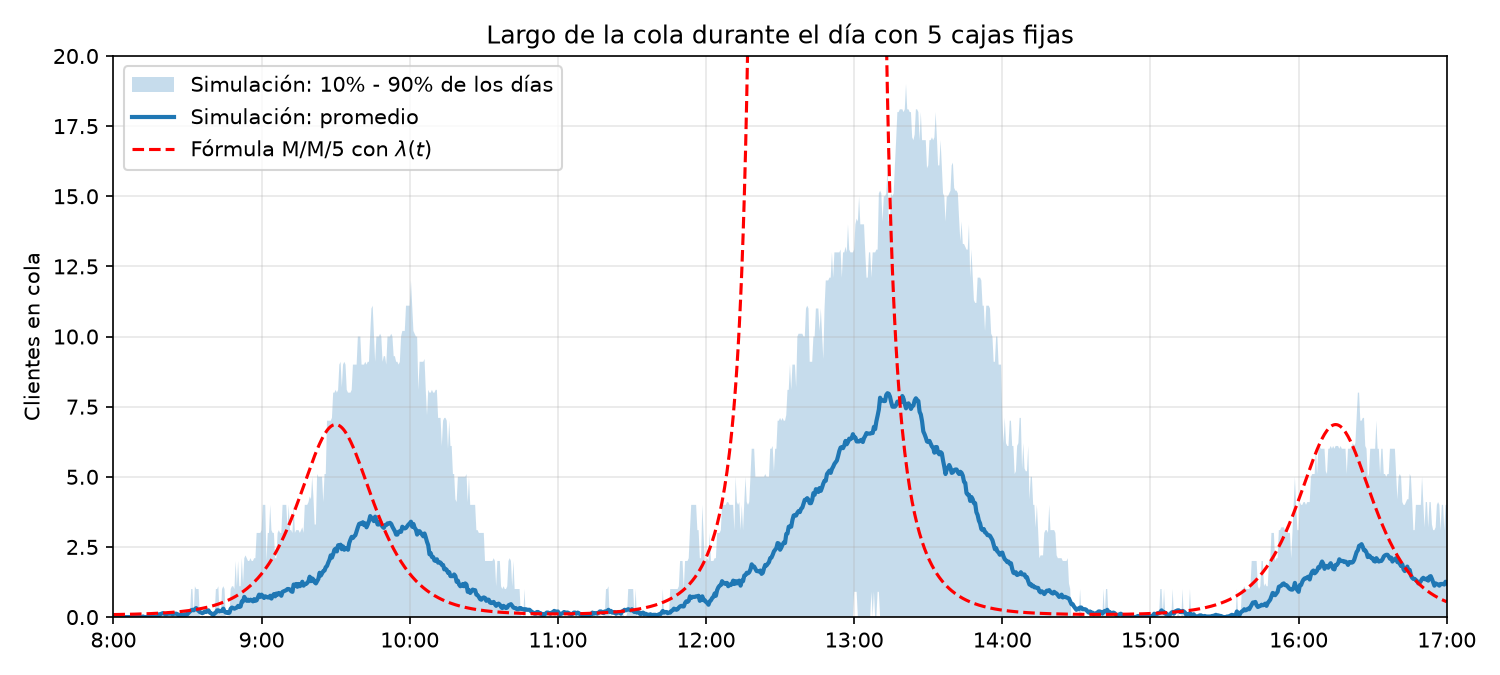
\includegraphics[width=0.95\textwidth]{esc3_cola_dia.png}
\caption{Clientes en la fila durante el día con 5 cajas fijas (50 días simulados) comparado con la fórmula estacionaria evaluada con $\lambda(t)$.}
\label{fig:coladia}
\end{figure}

\paragraph{Planes de personal.} La Tabla~\ref{tab:planes} compara cuatro planes. Tener 5
cajeros fijos es el plan con menos horas, pero un 7\,\% de los clientes espera más de 10
minutos y la espera máxima de cada día es en promedio 15 minutos. Pasar a 6 fijos
resuelve el problema pero cuesta 9 horas-cajero más. Los planes con refuerzo logran un
servicio parecido al de 6 fijos con menos horas: con 4 fijos y 2 de refuerzo
se usan 47 horas (solo 2 más que con 5 fijos) y la espera promedio baja de 2.39 a 0.97
minutos. La Figura~\ref{fig:esperahora} muestra de dónde viene la mejora: el plan de 5
fijos funciona bien fuera de los picos, pero en el almuerzo la espera promedio llega a 8
minutos.

\begin{table}[H]
\centering
\caption{Comparación de planes de personal en el día con horas pico (50 días simulados). Tiempos en minutos.}
\label{tab:planes}
\small
\begin{tabular}{@{}lrrrrrr@{}}
\toprule
Plan & Horas- & $W_q$ & IC 95\,\% & Percentil & Espera & \% espera \\
 & cajero & & ($\pm$) & 95 & máxima & $> 10$ min \\
\midrule
5 fijos & 45.0 & 2.39 & 0.38 & 10.76 & 15.25 & 7.15 \\
6 fijos & 54.0 & 0.68 & 0.14 & 4.18 & 7.45 & 0.63 \\
4 fijos + 2 refuerzo & 47.0 & 0.97 & 0.16 & 5.31 & 9.59 & 1.11 \\
5 fijos + 1 refuerzo & 50.5 & 0.74 & 0.14 & 4.47 & 7.87 & 0.66 \\
\bottomrule
\end{tabular}
\end{table}

\begin{figure}[H]
\centering
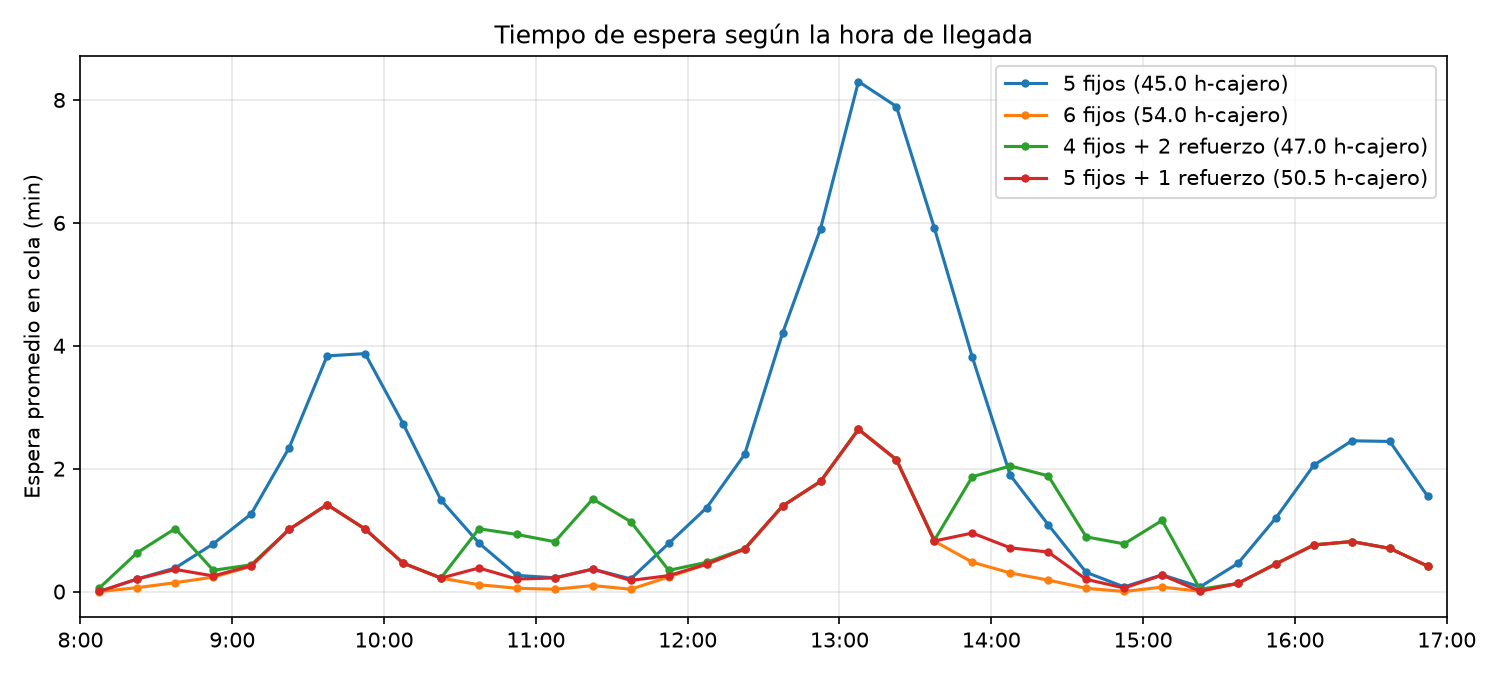
\includegraphics[width=0.95\textwidth]{esc3_espera_por_hora.png}
\caption{Espera promedio según la hora de llegada para cada plan de personal.}
\label{fig:esperahora}
\end{figure}

En todos los planes el último cliente termina de ser atendido entre 11 y 12 minutos
después del cierre, en promedio, por las personas que todavía estaban en la fila a las
17:00.

\subsection{Escenario 4: variabilidad del servicio}
En este escenario la media del servicio es la misma en todos los casos y solo cambia su
variabilidad. Los resultados (Tablas~\ref{tab:mg1} y \ref{tab:mgc}, Figura~\ref{fig:var})
muestran que la espera crece linealmente con $C_s^2$, como predice \eqref{eq:pk}. Con un
servidor, la fórmula de Pollaczek-Khinchine coincide con la simulación en todos los casos
(error máximo de 2.4\,\%, siempre dentro del intervalo de confianza). Pasar de un servicio
exponencial a uno determinista reduce la espera a la mitad (de 12.5 a 6.3 minutos), y un
servicio muy variable ($C_s^2 = 4$) la multiplica por 2.5.

\begin{table}[H]
\centering
\caption{M/G/1 con $\rho = 0.833$ y servicio promedio de 2.5 min.}
\label{tab:mg1}
\small
\begin{tabular}{@{}lrrrrr@{}}
\toprule
Distribución & $C_s^2$ & $W_q$ P-K (min) & $W_q$ simulado (min) & IC 95\,\% ($\pm$) & Error (\%) \\
\midrule
Determinista & 0.000 & 6.250 & 6.263 & 0.220 & 0.21 \\
Uniforme & 0.213 & 7.583 & 7.687 & 0.238 & 1.37 \\
Gamma ($k=2$) & 0.500 & 9.375 & 9.302 & 0.324 & 0.78 \\
Exponencial & 1.000 & 12.500 & 12.795 & 0.575 & 2.36 \\
Gamma ($k=0.5$) & 2.000 & 18.750 & 18.611 & 0.903 & 0.74 \\
Gamma ($k=0.25$) & 4.000 & 31.250 & 31.505 & 1.816 & 0.82 \\
\bottomrule
\end{tabular}
\end{table}

Con 5 servidores la aproximación de Allen-Cunneen funciona bien para $C_s^2 \le 1$
(diferencias de hasta 2.1\,\%), pero empieza a sobreestimar la espera cuando el servicio es
muy variable: con $C_s^2 = 4$ la diferencia es de 5.7\,\% y el valor aproximado queda fuera
del intervalo de confianza. Este es un caso donde la simulación da una respuesta más
confiable que la fórmula disponible.

\begin{table}[H]
\centering
\caption{M/G/5 con $\rho = 0.833$ y servicio promedio de 5 min.}
\label{tab:mgc}
\small
\begin{tabular}{@{}lrrrrr@{}}
\toprule
Distribución & $C_s^2$ & $W_q$ Allen-Cunneen & $W_q$ simulado & IC 95\,\% ($\pm$) & Diferencia (\%) \\
\midrule
Determinista & 0.000 & 1.860 & 1.899 & 0.039 & 2.01 \\
Uniforme & 0.213 & 2.257 & 2.307 & 0.047 & 2.15 \\
Gamma ($k=2$) & 0.500 & 2.791 & 2.794 & 0.080 & 0.10 \\
Exponencial & 1.000 & 3.721 & 3.691 & 0.118 & 0.80 \\
Gamma ($k=0.5$) & 2.000 & 5.581 & 5.416 & 0.253 & 3.06 \\
Gamma ($k=0.25$) & 4.000 & 9.302 & 8.798 & 0.416 & 5.73 \\
\bottomrule
\end{tabular}
\end{table}

\begin{figure}[H]
\centering
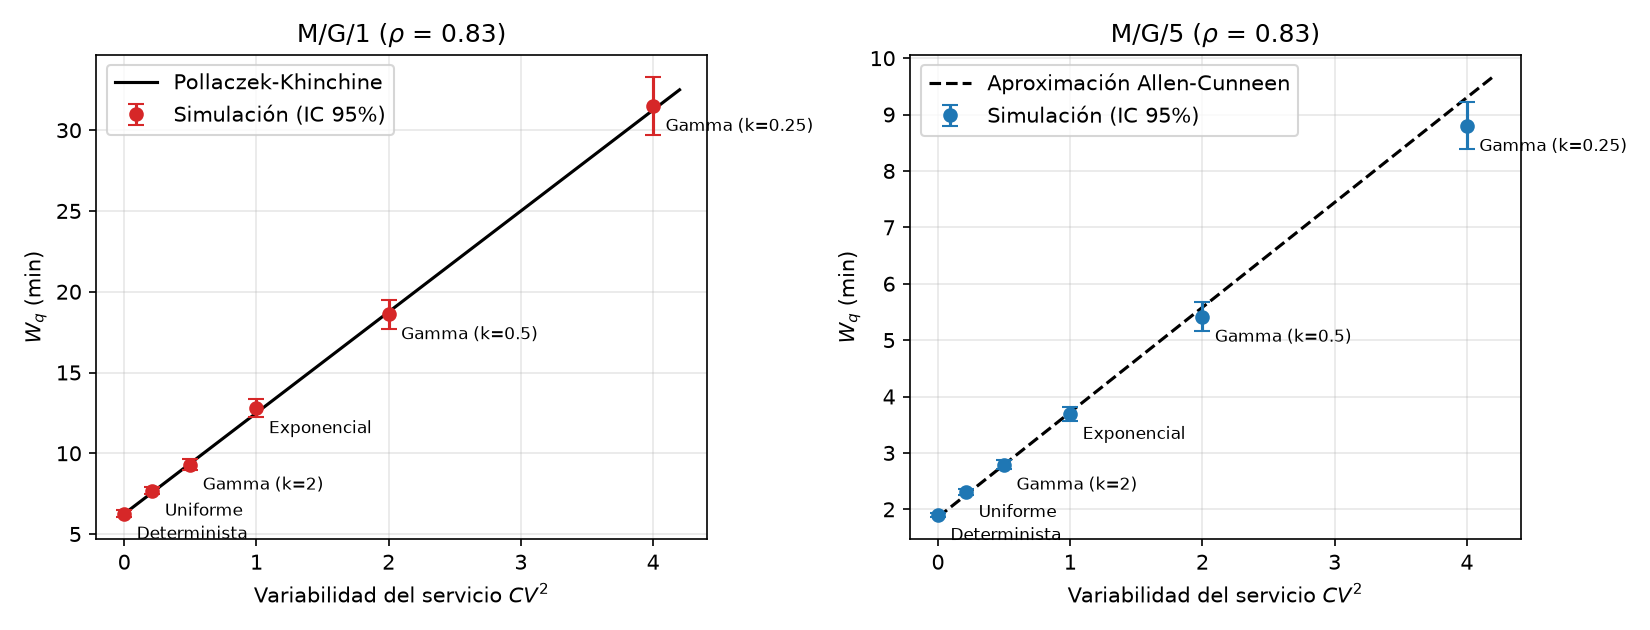
\includegraphics[width=\textwidth]{esc4_variabilidad.png}
\caption{Tiempo en cola en función de la variabilidad del servicio. Izquierda: M/G/1 contra Pollaczek-Khinchine. Derecha: M/G/5 contra la aproximación de Allen-Cunneen.}
\label{fig:var}
\end{figure}

\subsection{Escenario 5: soluciones óptimas}

\paragraph{Caso estacionario.} La Tabla~\ref{tab:costo} y la Figura~\ref{fig:costo} muestran
el costo total por hora para $c = 5,\dots,10$. Con pocas cajas domina el costo de espera,
que cae muy rápido al agregar cajeros, y con muchas cajas domina el costo de los
cajeros, que crece de forma lineal. El mínimo está en $\boldsymbol{c^* = 6}$, con un costo
de Q316 por hora, contra Q417 con 5 cajas y Q330 con 7. La simulación y la teoría
coinciden en todos los puntos.

\begin{table}[H]
\centering
\caption{Costo total por hora en el caso estacionario ($C_s = $ Q45/h, $C_w = $ Q60/h).}
\label{tab:costo}
\small
\begin{tabular}{@{}crrrrr@{}}
\toprule
$c$ & Cajeros (Q/h) & Espera teórica (Q/h) & Total teórico (Q/h) & Total simulado (Q/h) & IC 95\,\% ($\pm$) \\
\midrule
5 & 225 & 186.04 & 411.04 & 416.81 & 10.65 \\
\textbf{6} & \textbf{270} & \textbf{44.61} & \textbf{314.61} & \textbf{316.36} & \textbf{2.39} \\
7 & 315 & 14.10 & 329.10 & 329.72 & 0.83 \\
8 & 360 & 4.70 & 364.70 & 364.91 & 0.34 \\
9 & 405 & 1.55 & 406.55 & 406.65 & 0.15 \\
10 & 450 & 0.49 & 450.49 & 450.54 & 0.08 \\
\bottomrule
\end{tabular}
\end{table}

\begin{figure}[H]
\centering
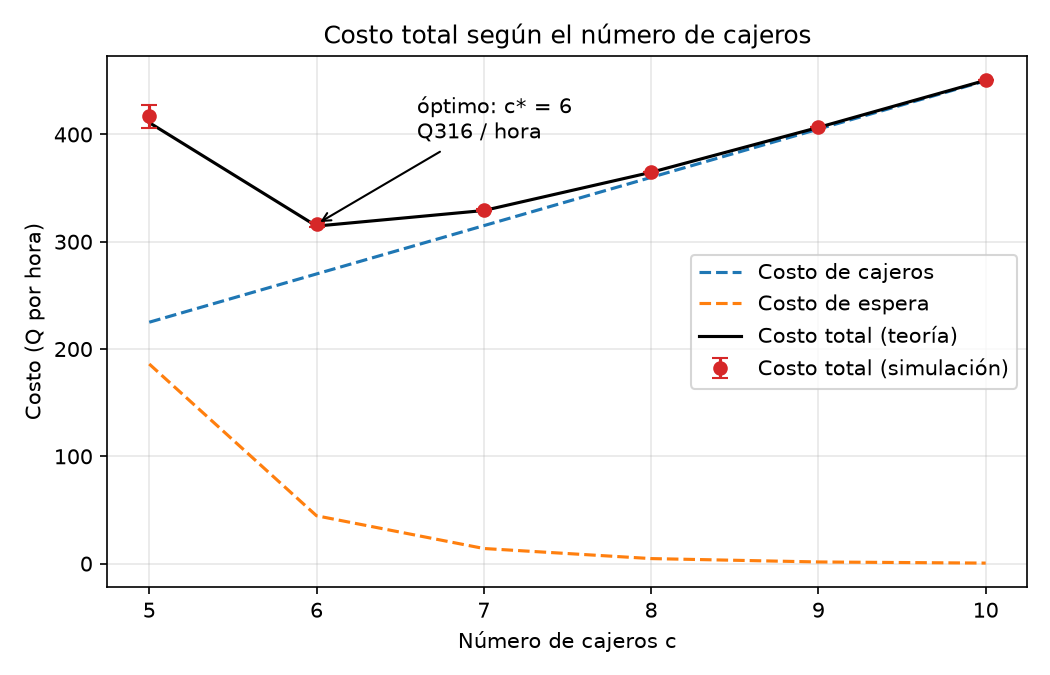
\includegraphics[width=0.7\textwidth]{esc5_costo_estacionario.png}
\caption{Costo de cajeros, costo de espera y costo total según el número de cajeros.}
\label{fig:costo}
\end{figure}

\paragraph{Sensibilidad.} Como el costo de espera $C_w$ es el parámetro más difícil de
estimar, calculamos el $c^*$ para distintos valores de la razón $C_w/C_s$
(Figura~\ref{fig:sens}). El óptimo es 6 cajeros mientras la razón esté entre 0.43 y 1.97;
en nuestro caso base la razón es 1.33, así que la decisión no depende mucho del valor
exacto de $C_w$. El óptimo sube a 7 cajeros si la espera se valora en más de 1.97 veces
el costo de un cajero, a 8 a partir de 6.4 y a 9 a partir de 19.4. Como el $c^*$ crece de
forma escalonada y lenta, aun si $C_w$ fuera cuatro veces mayor que el supuesto el óptimo
solo subiría a 7 cajeros.

\begin{figure}[H]
\centering
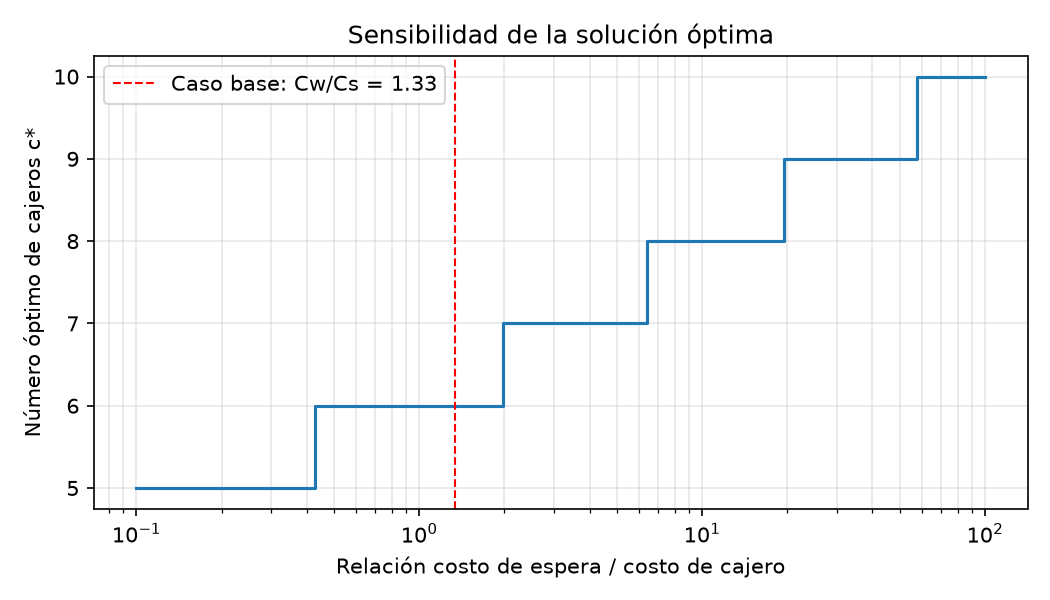
\includegraphics[width=0.65\textwidth]{esc5_sensibilidad.png}
\caption{Número óptimo de cajeros en función de la razón $C_w/C_s$.}
\label{fig:sens}
\end{figure}

\paragraph{Día con horas pico.} Para el día completo evaluamos 16 planes con los mismos 50
días simulados. La Tabla~\ref{tab:planesdia} muestra los ocho de menor costo y la
Figura~\ref{fig:heat} los 16. El plan óptimo es \textbf{4 cajeros fijos más 2 de refuerzo},
con un costo de Q2,566 por día. Los valores de esta tabla son un poco distintos a los de
la Tabla~\ref{tab:planes} porque se calcularon con otro conjunto de días simulados, pero
quedan dentro de los intervalos de confianza.

\begin{table}[H]
\centering
\caption{Los ocho planes de menor costo para el día con horas pico (50 días simulados).}
\label{tab:planesdia}
\small
\begin{tabular}{@{}ccrrrrrr@{}}
\toprule
Fijos & Refuerzo & Horas- & $W_q$ & \% espera & Costo & Costo & Costo total \\
 & & cajero & (min) & $> 10$ min & cajeros (Q) & espera (Q) & (Q/día) \\
\midrule
\textbf{4} & \textbf{2} & \textbf{47.0} & \textbf{1.16} & \textbf{2.16} & \textbf{2,115} & \textbf{451} & \textbf{2,566 $\pm$ 95} \\
4 & 3 & 52.5 & 0.57 & 0.50 & 2,363 & 222 & 2,584 $\pm$ 44 \\
5 & 1 & 50.5 & 0.92 & 1.69 & 2,273 & 357 & 2,630 $\pm$ 88 \\
5 & 2 & 56.0 & 0.36 & 0.23 & 2,520 & 142 & 2,662 $\pm$ 39 \\
6 & 0 & 54.0 & 0.84 & 1.60 & 2,430 & 327 & 2,757 $\pm$ 84 \\
3 & 3 & 43.5 & 2.09 & 5.95 & 1,958 & 813 & 2,770 $\pm$ 131 \\
6 & 1 & 59.5 & 0.30 & 0.17 & 2,678 & 118 & 2,795 $\pm$ 37 \\
5 & 3 & 61.5 & 0.18 & 0.05 & 2,768 & 71 & 2,838 $\pm$ 18 \\
\midrule
5 & 0 & 45.0 & 2.65 & 8.03 & 2,025 & 1,029 & 3,054 $\pm$ 196 \\
\bottomrule
\end{tabular}
\end{table}

\begin{figure}[H]
\centering
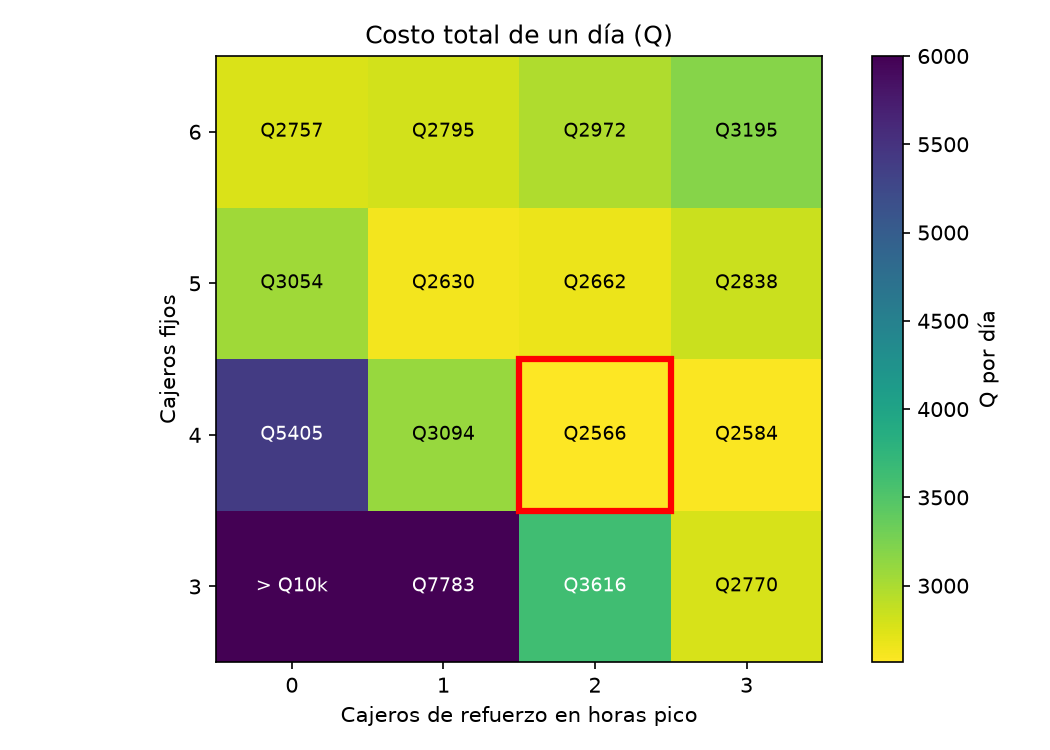
\includegraphics[width=0.6\textwidth]{esc5_planes_dia.png}
\caption{Costo total de un día para cada combinación de cajeros fijos y de refuerzo. El recuadro marca el óptimo.}
\label{fig:heat}
\end{figure}

Los intervalos de los primeros planes se traslapan, así que hicimos una comparación
pareada aprovechando que todos se evaluaron con los mismos días. La diferencia entre
4+3 y 4+2 fue de Q$18.0 \pm 56.6$, que no es significativa: los dos planes son
prácticamente equivalentes en costo, aunque 4+3 da mejor servicio (0.5\,\% de clientes
con más de 10 minutos de espera contra 2.2\,\%). En cambio, 5+1 cuesta Q$63.3 \pm 19.3$ más
por día y 5+2 cuesta Q$96.0 \pm 59.3$ más, y ambas diferencias sí son significativas.
Comparado con el plan de 5 cajeros fijos (el que se elegiría usando la tasa promedio), el
plan óptimo ahorra unos Q490 por día y reduce a menos de la mitad la espera
promedio.

\subsection{Visualización de la simulación}
Además de las gráficas, el archivo \texttt{animacion.py} genera una animación de un día
completo. En ella se ven los cajeros (verde si están atendiendo, gris si están
libres y blanco si están fuera de turno), los clientes en la fila y, abajo, el largo de la
fila acumulado durante el día. La Figura~\ref{fig:anim} muestra el cuadro de la 1:00 p.m.
para dos planes, simulados con el mismo día de llegadas.

\begin{figure}[H]
\centering
\begin{subfigure}{\textwidth}
\centering
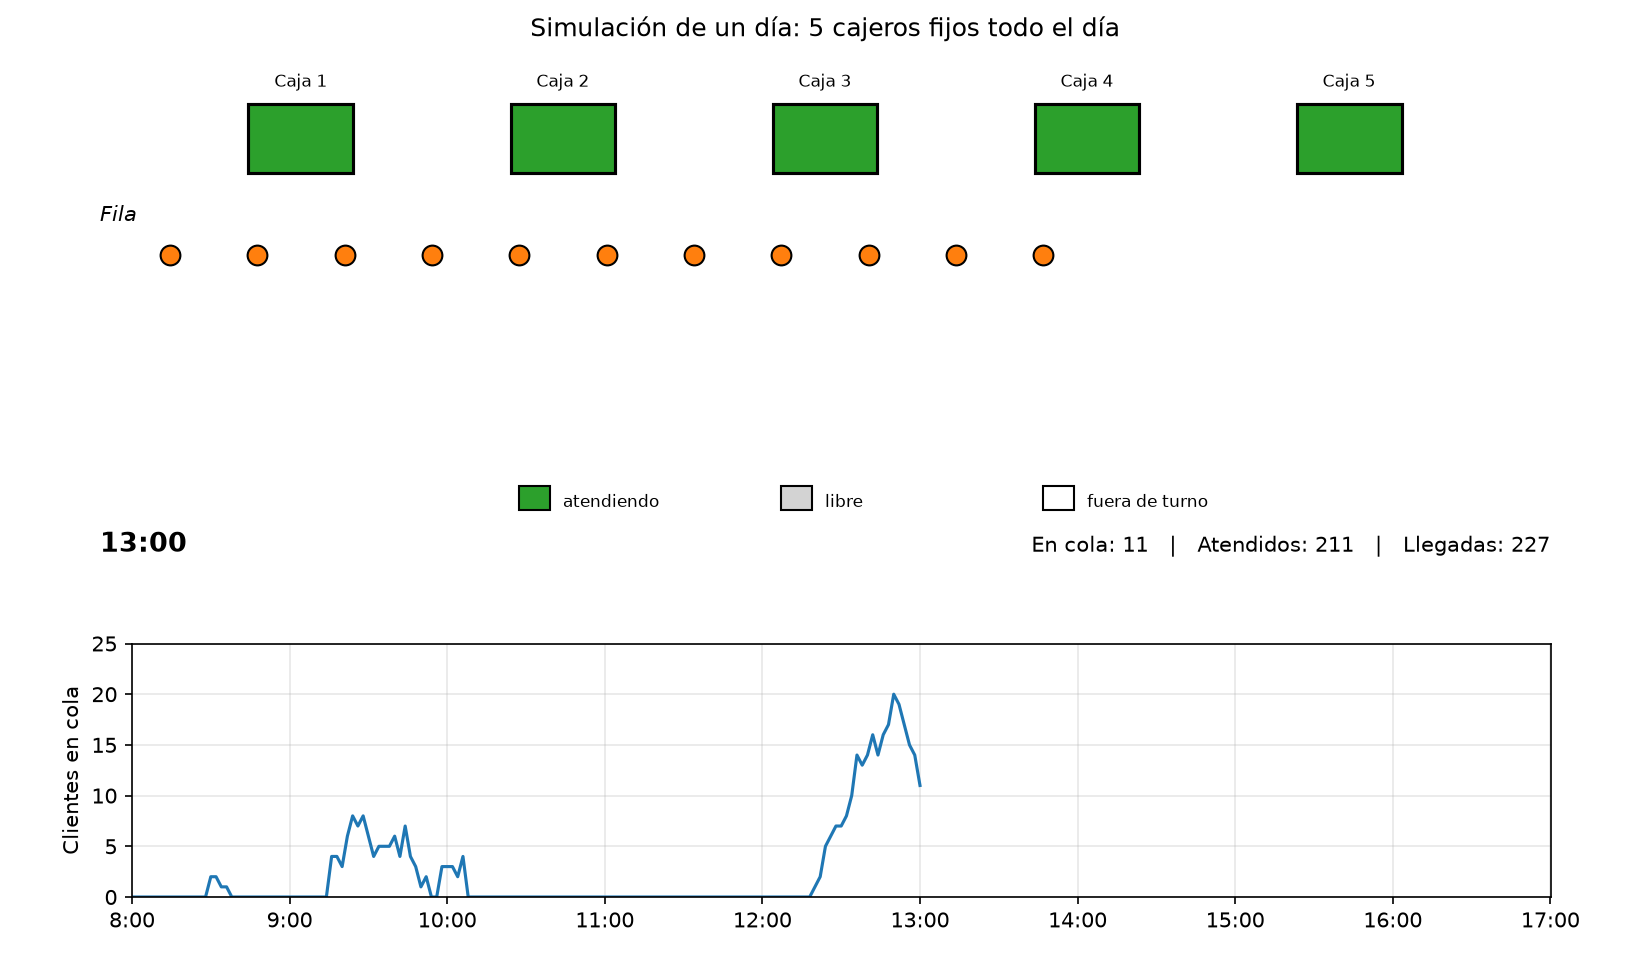
\includegraphics[width=0.85\textwidth]{animacion_5_fijos_13h.png}
\caption{5 cajeros fijos.}
\end{subfigure}

\vspace{0.3cm}
\begin{subfigure}{\textwidth}
\centering
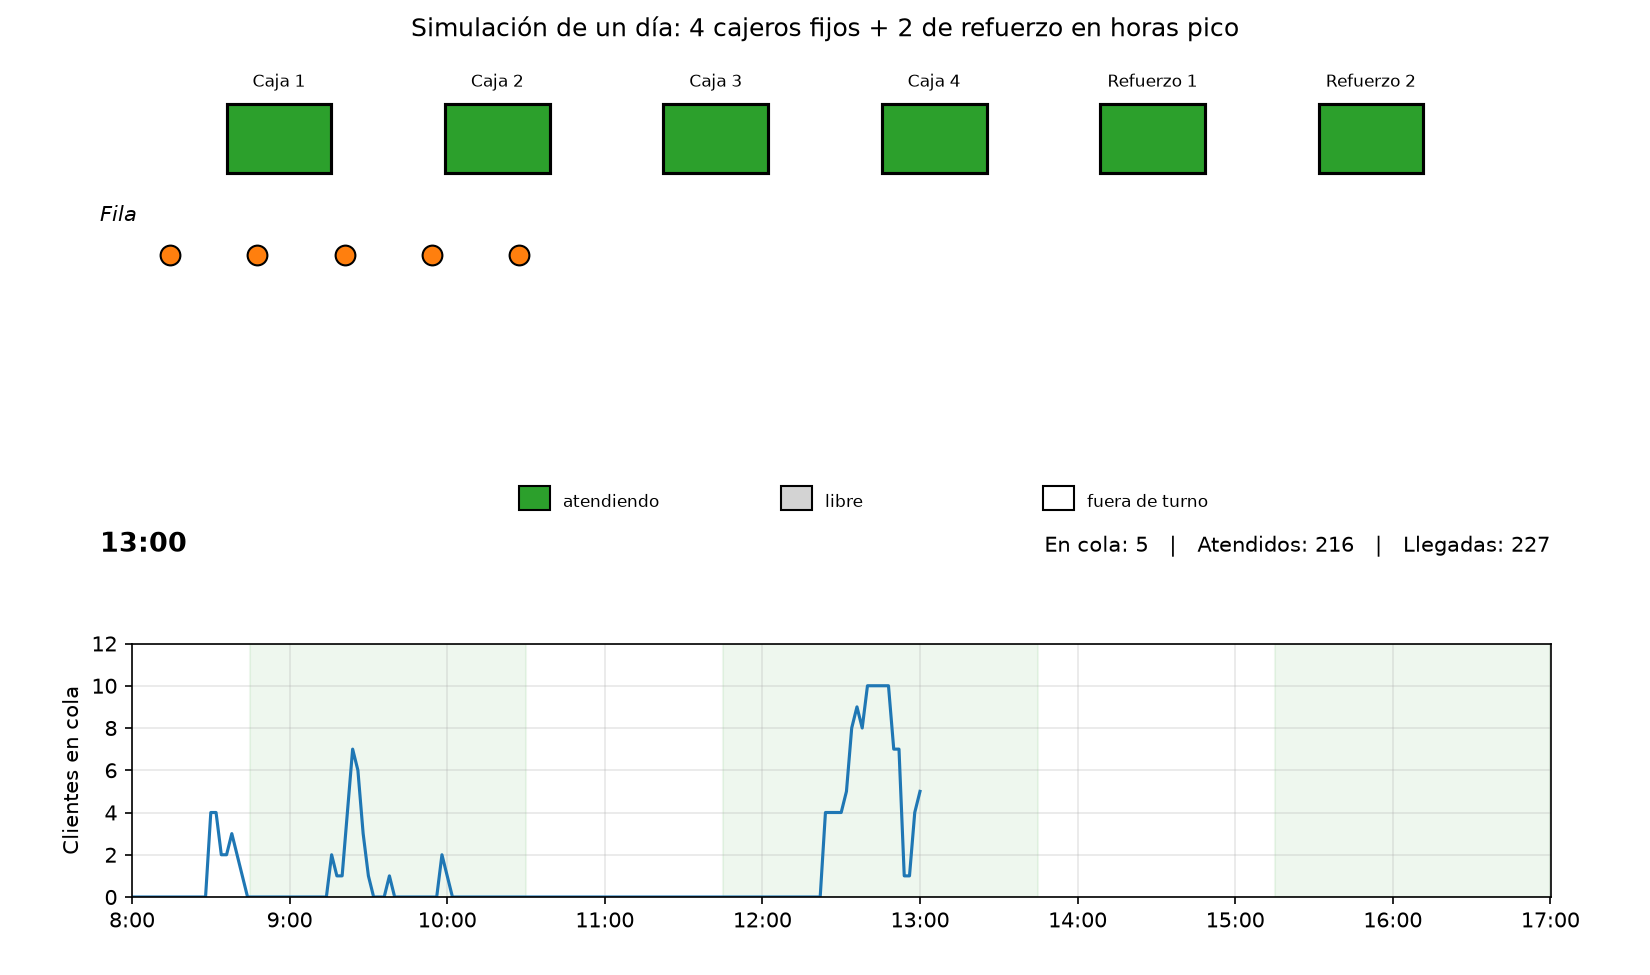
\includegraphics[width=0.85\textwidth]{animacion_4_fijos_2_refuerzo_13h.png}
\caption{4 cajeros fijos y 2 de refuerzo.}
\end{subfigure}
\caption{Cuadro de la animación a la 1:00 p.m. para el mismo día simulado con dos planes distintos.}
\label{fig:anim}
\end{figure}

% ------------------------------------------------------------------
\section{Discusión}
% ------------------------------------------------------------------
La primera parte del trabajo muestra que el simulador reproduce los resultados teóricos
de M/M/1, M/M/$c$ y M/G/1 con errores pequeños y siempre dentro de los intervalos de
confianza. Esto nos da confianza para usarlo en los casos donde no hay fórmula, que son
justamente los más interesantes. También aprendimos que la calidad de la estimación
depende mucho del diseño del experimento: cerca de la saturación hace falta simular
mucho más tiempo y descartar un calentamiento más largo, porque de lo contrario la
simulación subestima la espera.

El escenario 3 es el que mejor muestra para qué sirve la simulación. Con la tasa
promedio, la fórmula de M/M/5 sugiere que 5 cajas son suficientes, con 1.35 minutos de
espera. La simulación muestra que en realidad la espera es casi el doble y que hay un
rato al mediodía en el que el sistema está saturado. Usar la fórmula hora por hora
tampoco funciona, porque no toma en cuenta que la fila se acumula y tarda en vaciarse.
Esto coincide con lo que se reporta en la literatura sobre dimensionamiento de personal
con demanda cíclica \cite{green}.

Otro resultado importante es que la forma de organizar el servicio pesa tanto como el
número de cajeros. Con las mismas 6 cajas, pasar de filas separadas a una fila única
reduce la espera de 11.5 a 0.9 minutos. Del mismo modo, reducir la variabilidad del
servicio (por ejemplo, con procesos más estandarizados) baja la espera sin contratar a
nadie: un servicio determinista tiene la mitad de espera que uno exponencial con la misma
media.

En cuanto a las limitaciones, los costos $C_s$ y $C_w$ son supuestos nuestros y no datos
reales de un banco. El análisis de sensibilidad muestra que el óptimo estacionario no
cambia mientras la razón $C_w/C_s$ esté entre 0.43 y 1.97, pero sería mejor estimar $C_w$
con datos, por ejemplo midiendo cuántos clientes se van sin ser atendidos. Tampoco
modelamos el abandono de la fila, clientes con distintos tipos de trámite ni pausas de los
cajeros, y la forma de $\lambda(t)$ la propusimos nosotros. Con datos reales de llegadas
habría que ajustar $\lambda(t)$ antes de usar los resultados para tomar decisiones.

% ------------------------------------------------------------------
\section{Conclusiones}
% ------------------------------------------------------------------
\begin{enumerate}
  \item El simulador por eventos discretos reproduce las fórmulas teóricas de M/M/1,
        M/M/$c$ (Erlang C) y M/G/1 (Pollaczek-Khinchine), con errores relativos de 4\,\% o
        menos en todas las medidas y con los valores teóricos dentro de los intervalos de
        confianza del 95\,\%. La ley de Little se cumple en las corridas simuladas.
  \item Los tiempos generados con Mersenne Twister y transformada inversa pasan las
        pruebas de Kolmogorov-Smirnov y $\chi^2$ ($p > 0.6$), y el método de
        \emph{thinning} genera el proceso no homogéneo con la eficiencia esperada (0.588
        contra 0.591 teórica).
  \item Cuando la demanda varía durante el día, las fórmulas estacionarias no son
        confiables: con 5 cajas la fórmula con la tasa promedio predice 1.35 minutos de
        espera y la simulación da 2.39 minutos, con filas de más de 15 personas en el
        almuerzo.
  \item En el caso estacionario (50 clientes por hora, 5 minutos por atención) el número
        óptimo de cajeros es $c^* = 6$, con un costo de Q316 por hora. Este resultado se
        mantiene para cualquier razón $C_w/C_s$ entre 0.43 y 1.97.
  \item Para el día con horas pico el plan óptimo es 4 cajeros fijos más 2 de refuerzo
        en los picos, con un costo de Q2,566 por día. Ahorra unos Q490 diarios frente a
        tener 5 cajeros fijos y reduce la espera promedio a menos de la mitad. El plan 4+3
        cuesta prácticamente lo mismo y da un mejor servicio.
  \item Con la misma cantidad de cajeros, una fila única reduce la espera promedio de
        11.5 a 0.9 minutos respecto a tener una fila por caja.
\end{enumerate}

% ------------------------------------------------------------------
\section{Sugerencias y trabajo futuro}
% ------------------------------------------------------------------
\begin{itemize}
  \item Usar una sola fila para todas las cajas, ya que es la mejora más grande y no
        tiene costo.
  \item Programar personal de refuerzo en las horas pico en lugar de aumentar el número
        de cajeros fijos durante todo el día.
  \item Estandarizar los trámites para reducir la variabilidad del tiempo de atención.
  \item Estimar $\lambda(t)$ y la distribución del servicio con datos reales de una
        agencia, y estimar el costo de espera a partir de la tasa de abandono.
  \item Extender el modelo con abandono de la fila, distintos tipos de clientes
        (por ejemplo, una fila preferencial) y optimizar también los horarios de las
        ventanas de refuerzo, no solo el número de cajeros.
\end{itemize}

% ------------------------------------------------------------------
\begin{thebibliography}{9}
% ------------------------------------------------------------------
\bibitem{allen} Allen, A. O. (1990). \emph{Probability, Statistics, and Queueing Theory with Computer Science Applications} (2.\textsuperscript{a} ed.). Academic Press.
\bibitem{green} Green, L. V., Kolesar, P. J. y Soares, J. (2001). Improving the SIPP approach for staffing service systems that have cyclic demands. \emph{Operations Research}, 49(4), 549--564.
\bibitem{gross} Gross, D., Shortle, J. F., Thompson, J. M. y Harris, C. M. (2008). \emph{Fundamentals of Queueing Theory} (4.\textsuperscript{a} ed.). Wiley.
\bibitem{law} Law, A. M. (2015). \emph{Simulation Modeling and Analysis} (5.\textsuperscript{a} ed.). McGraw-Hill.
\bibitem{lewis} Lewis, P. A. W. y Shedler, G. S. (1979). Simulation of nonhomogeneous Poisson processes by thinning. \emph{Naval Research Logistics Quarterly}, 26(3), 403--413.
\bibitem{little} Little, J. D. C. (1961). A proof for the queuing formula: $L = \lambda W$. \emph{Operations Research}, 9(3), 383--387.
\bibitem{mt} Matsumoto, M. y Nishimura, T. (1998). Mersenne Twister: a 623-dimensionally equidistributed uniform pseudo-random number generator. \emph{ACM Transactions on Modeling and Computer Simulation}, 8(1), 3--30.
\bibitem{ross} Ross, S. M. (2013). \emph{Simulation} (5.\textsuperscript{a} ed.). Academic Press.
\bibitem{taha} Taha, H. A. (2017). \emph{Investigación de operaciones} (10.\textsuperscript{a} ed.). Pearson.
\end{thebibliography}

% ------------------------------------------------------------------
\appendix
\section{Estructura del código}
% ------------------------------------------------------------------
El código se ejecuta con Python 3 y las librerías indicadas en \texttt{requirements.txt}.
El archivo \texttt{correr\_todo.py} corre todos los escenarios en orden (tarda alrededor de
dos minutos); las gráficas se guardan en la carpeta \texttt{figuras} y las tablas en
\texttt{resultados}.

\begin{table}[H]
\centering
\small
\begin{tabular}{@{}lp{10cm}@{}}
\toprule
Archivo & Contenido \\
\midrule
\texttt{simulador.py} & Generación de variables aleatorias, simulación de la cola (con y sin turnos), cálculo de medidas, réplicas, intervalos de confianza y fórmulas teóricas. \\
\texttt{modelo\_banco.py} & Tasa de llegadas $\lambda(t)$, ventanas de refuerzo y planes de turnos de la agencia. \\
\texttt{esc1\_mm1.py} & Escenario 1: pruebas de ajuste, validación de M/M/1 y barrido de $\rho$. \\
\texttt{esc2\_mmc.py} & Escenario 2: M/M/$c$, distribución de la espera y fila única contra filas separadas. \\
\texttt{esc3\_hora\_pico.py} & Escenario 3: día con horas pico y comparación de planes. \\
\texttt{esc4\_servicio.py} & Escenario 4: M/G/1 y M/G/5 con distintas distribuciones de servicio. \\
\texttt{esc5\_optimizacion.py} & Escenario 5: costo total, sensibilidad y búsqueda del mejor plan. \\
\texttt{animacion.py} & Animación de un día (\texttt{python animacion.py mostrar} la abre en una ventana). \\
\bottomrule
\end{tabular}
\end{table}

\end{document}
